% !TeX program = xelatex
% Main manuscript: Elsevier CAS single-column, Chinese working draft.
% Original CAS sample and the previous manuscript are preserved in archive/.
\providecommand{\PaperRoot}{./}
\makeatletter
\edef\input@path{{\PaperRoot}{\PaperRoot template/}}
\makeatother
\PassOptionsToPackage{no-math}{fontspec}
\documentclass[a4paper]{cas-sc}
% CAS enables fleqn internally; retain right-hand numbers but center displays.
\makeatletter
\@fleqnfalse
\makeatother
\usepackage[UTF8,scheme=plain,fontset=windows]{ctex}
\usepackage[numbers,sort&compress]{natbib}
\usepackage{bm,tabularx,longtable}
\usepackage{algorithm,algpseudocode}
\usepackage{tikz}
\usetikzlibrary{arrows.meta,positioning,fit}
\usepackage{placeins,needspace,xr}\externaldocument{build/paper_draft}
\hypersetup{unicode=true,hidelinks}
\pdfstringdefDisableCommands{\def\\{ }}
\graphicspath{{\PaperRoot}}
\numberwithin{equation}{section}
\numberwithin{figure}{section}
\numberwithin{table}{section}
\renewcommand{\figurename}{图}
\renewcommand{\tablename}{表}
\renewcommand{\abstractname}{摘要}
\floatname{algorithm}{算法}
\algrenewcommand{\algorithmicrequire}{\textbf{输入：}}
\renewcommand{\refname}{参考文献}
\newcommand{\R}{\mathbb R}
\newcommand{\C}{\mathbb C}
\newcommand{\E}{\mathbb E}
\newcommand{\Rea}{\operatorname{Re}}
\newcommand{\tr}{\operatorname{tr}}
\newcommand{\diag}{\operatorname{diag}}
\setlength{\emergencystretch}{2em}
\widowpenalty=10000
\clubpenalty=10000
% No author information has been supplied. Keep the draft footer factual.
\ExplSyntaxOn
\RenewDocumentCommand\MaketitleBox{O{}}
 {\group_begin:\use:c{@title}\par\group_end:\vspace{12pt}}
% Local presentation override: center both short and multiline captions.
\cs_set_protected:Npn \__make_tbl_caption:nn #1#2
  {
    \l_tbl_align_tl
    \skip_vertical:N \l_tbl_abovecap_skip
    \parbox{\l_tbl_width_dim}
      {\centering\sffamily\small
       \textbf{\color{scolor}#1}\par #2\par\vskip4pt}
    \skip_vertical:N \l_tbl_belowcap_skip
  }
\cs_set_protected:Npn \__make_fig_caption:nn #1#2
  {
    \l_fig_align_tl
    \skip_vertical:N \l_fig_abovecap_skip
    \parbox{\l_fig_width_dim}
      {\centering\sffamily\small
       \textbf{\color{scolor}#1:}~#2\par}
    \skip_vertical:N \l_fig_belowcap_skip
  }
\cs_set:Npn \__first_footerline:
  { \small\rmfamily\itshape Signal~Processing\quad 中文初稿 }
% CAS 2.4 uses a zero-width keyword overlay; stretchable glue preserves its
% position while avoiding the template's artificial overfull-box diagnostic.
\exp_args:Nc \patchcmd { environment~Abstract~code }
  { \box \g_stm_key_box } { \box \g_stm_key_box \hss }
  { } { \PackageError{paper}{CAS~abstract~compatibility~patch~failed}{} }
\cs_new_eq:NN \paper_printorcid: \printorcid
\RenewDocumentCommand \printorcid { }
  { \seq_if_empty:NF \g_stm_orcid_seq { \paper_printorcid: } }
\ExplSyntaxOff
\begin{document}
\let\WriteBookmarks\relax
\shorttitle{直接定位论文补充材料}
\shortauthors{}
\title[mode=title]{未知宽带强弱重叠源的高效直接定位：补充材料}
\maketitle
\renewcommand{\thesection}{S\arabic{section}}
本文件保存主稿压缩后移出的基线准则、数值核验及辅助结果；实验输入和结果不变。新16个布局的完整精度坐标保存在\texttt{data/submission/new\_layouts.csv}；英文补充材料第S1节给出坐标表和编号映射。几何与波形种子分别为20261020071和20261020072，随机实现编号为1000--1004。正文采用一基布局编号，减一即为保存结果中的零基编号。


% BEGIN sections/appendix
\section{比较方法在本模型下的准则}\label{app:baselines}
\subsection{单源谱、MUSIC及MVDR-known}
LS取峰使用式\eqref{eq:single}，每个位置分别按单源模型评分。MUSIC和MVDR则需要从观测估计空间统计量。为此，将同一记录划分为$S$个不重叠片段，各片段长度为$N_s=N/S$。令$\bm z_{bf}\in\C^L$表示第$b$段在频率$f$处的多站DFT观测，$b=1,\ldots,S$。各段采用共同的频率轴，并在该轴上选择相同物理频带；样本协方差估计为
\begin{equation}
 \widehat{\bm C}_f=S^{-1}\sum_{b=1}^S\bm z_{bf}\bm z_{bf}^H .
\end{equation}
同一记录内的位置、传播关系和信号统计保持不变，各片段DFT用于构成同频快拍。零均值模型下，相关矩阵等于协方差矩阵，故上式不另减样本均值。完整记录与片段DFT分别按$1/N$和$1/N_s$归一化，对应噪声方差为$\sigma_t^2/N$和$\sigma_t^2/N_s$。分段提供更多统计快拍，同时降低频率分辨率、缩短单段时长。

MUSIC利用信号响应与噪声子空间的正交关系定位\cite{WeissAmar2005}。其通常要求$K<L$、源频域系数的协方差满秩、不同源的跨站响应线性独立，并采用空间白噪声模型。在两源均有非零功率的频点，独立源的总体协方差满足相应源秩条件；有限记录下的子空间估计精度还与功率差、有效快拍数及频点信号强度有关。本文采用逐频响应与宽带评分汇聚。

设$\bm E_{n,f}\in\C^{L\times(L-K)}$的列为$\widehat{\bm C}_f$最小$L-K$个特征值对应的单位正交特征向量。用已知源数$K$划分子空间，本文MUSIC适配版使用
\begin{align}
 S_{\mathrm{MU}}(\bm p)&=\left[\sum_f w_f
 \bm q_f(\bm p)^H\bm E_{n,f}\bm E_{n,f}^H\bm q_f(\bm p)\right]^{-1},\label{eq:music}\\
 \widetilde w_f&=\max\{\tr(\widehat{\bm C}_f)-L\sigma_t^2/N_s,0\},\quad
 w_f=\widetilde w_f/\sum_v\widetilde w_v .\nonumber
\end{align}
式中$\tr$为矩阵迹，$\widetilde w_f$为扣除期望噪声后的非负观测功率，$w_f$为归一化权重，$v$遍历保留频点。所有权重为零时使用均匀权重。该宽带汇聚使信号能量较高的频点发挥更大作用；带外频点不参与分解。

MVDR在保持候选响应不失真的条件下，最小化输出功率\cite{Capon1969}。令$\bm h_f\in\C^L$为复数合成权重，对加载后的协方差解
\begin{equation}
 \min_{\bm h_f}\ \bm h_f^H\bm C_{f,\delta}\bm h_f,
 \qquad \bm h_f^H\bm q_f(\bm p)=1.\label{eq:mvdrConstraint}
\end{equation}
最优输出功率为$[\bm q_f^H\bm C_{f,\delta}^{-1}\bm q_f]^{-1}$。将这一功率在保留频点上平均，得到MVDR-known评分：
\begin{align}
 \bm C_{f,\delta}&=\widehat{\bm C}_f+
 \delta\,\tr(\widehat{\bm C}_f)\bm I/L,\nonumber\\
 S_{\mathrm{MV}}(\bm p)&=F_s^{-1}\sum_f
 [\bm q_f(\bm p)^H\bm C_{f,\delta}^{-1}\bm q_f(\bm p)]^{-1} .\label{eq:mvdr}
\end{align}
这里$\delta>0$为无量纲相对加载量，加载项是平均对角功率$\tr(\widehat{\bm C}_f)/L$的$\delta$倍，用于缓解有限快拍下求逆不稳定的问题；$F_s$为片段频率轴上保留的频点数，区别于采样率$f_s$。约束中的响应和评分均使用同一单位范数向量$\bm q_f$。“known”表示采用已知相对传播响应；本宽带汇聚式与DPD-HR的原公式分别命名\cite{TirerWeiss2016}。

\subsection{有限分段的模型一致性}\label{app:segmentcheck}
为检查短窗近似，使用四类开发构型的0/15\,dB观测，共8条，直接读取仿真保存的无噪声源分量。在真实位置处构造$\bm A_f$，计算干净混合观测的最小二乘残差；这一步只核对观测模型，不搜索位置。对$S$段、每段$N_s=N/S$点，定义
\begin{equation}
 E_{\mathrm{win}}=\sum_{b=1}^{S}\sum_{f\in\mathcal F_s}
 \|\bm\Pi_{\bm A_f}^{\perp}\bm z_{bf}^{(0)}\|^2,\qquad
 E_{\mathrm n}=SF_s(L-K)\sigma_t^2/N_s ,
 \label{eq:windowdiagnostic}
\end{equation}
其中$\bm z_{bf}^{(0)}$为无噪声分段DFT，$\mathcal F_s$为该段长下保留的频点集合，$F_s=|\mathcal F_s|$。$E_{\mathrm n}$是相同投影后的白噪声期望能量；各频点$\bm A_f$均经检查满列秩。表\ref{tab:windowdiagnostic}使用各自段长、频率轴和DFT归一化，传播常数与原仿真一致。

\begin{table}[pos=H]\centering\small
\caption{8条开发观测的有限窗模型核验。占比为$E_{\mathrm{win}}$除以保留频点的干净混合观测能量，表中列出观测间范围。}\label{tab:windowdiagnostic}
\begin{tabular}{@{}lrrr@{}}\toprule
分段数 & 单段时长/$\mu$s & 残差占比/\% & $E_{\mathrm{win}}/E_{\mathrm n}$\\\midrule
1 & 163.84 & 0.209--0.382 & 0.035--0.882\\
4 & 40.96 & 0.756--1.387 & 0.126--3.210\\
8 & 20.48 & 1.529--2.854 & 0.238--6.611\\\bottomrule
\end{tabular}\end{table}
分段越短，截取共同观测窗造成的跨站频域偏差越明显。15\,dB的四条观测中，4段和8段的模型残差均超过预计投影后噪声能量。为区分这一偏差与定位失败，进一步在相同记录上比较矩形窗、周期Hann窗以及4096点Hann长窗的4个重叠帧。公共频带、原噪声与功率不变，窗化后的频域噪声方差按$\sigma_t^2\sum_n w[n]^2/N_s^2$计算，其中$w[n]$为实际窗；重叠帧不视为独立快拍。

15\,dB时，长Hann窗将模型残差与预计投影后噪声能量之比降至0.076--0.294，MUSIC与MVDR-known仍分别仅有1/4和0/4成功，与原矩形配置的失败身份一致；0\,dB时两者均为4/4成功。另将每源的无噪声分量投影到真实响应后，再加入原噪声，构造模型残差接近数值零的诊断数据，原7个失败方法--观测对仍未恢复。该对照使用真值，仅用于归因，不参加方法排名。

这组结果表明，有限窗模型误差并不足以解释所测失败；当前记录和强弱源条件下，谱评分与取峰流程仍存在恢复限制。上述诊断不改变正式基线配置，核心AP与BNOMP的受控比较继续使用同一完整记录。

\subsection{充分AP、多初值联合ML与GA}
充分AP对各源反复进行全域条件扫描与连续精修，以式\eqref{eq:profile}判断更新\cite{ChenHudsonYao2002}。它与MCJ-AP优化同一目标，但进行更多初值处理和全域核查。实验同时报告保存的早期解与最终停止时间，区分取得结果和完成核查的成本。

多初值联合ML从四个唯一的谱峰组合和四个Sobol低差异序列给出的空间覆盖组合出发，以有界L-BFGS-B最小化$J$，输出最小残差解。候选组合的无序重复在初始化阶段删除。遗传算法（GA）将两个源的四个坐标编码为一个实数个体，在相同目标$J$上进行锦标赛选择、模拟二进制交叉和多项式变异\cite{DebAgrawal1995}，保留4个精英，最后作联合连续精修。锦标赛规模为3，交叉概率为0.9、分布指数为15，每维变异概率为0.25、分布指数为20。这些参数控制个体选择与扰动范围；总体成本由种群规模、代数和实际目标调用共同决定。

\subsection{多频共享功率SBL}
稀疏贝叶斯学习（SBL）在离散位置字典上估计稀疏源功率。令$\bm g_j\in\Omega$为第$j$个字典位置，$\bm D_f=[\bm q_f(\bm g_1),\ldots,\bm q_f(\bm g_G)]\in\C^{L\times G}$。逐频系数$\bm z_f\in\C^G$采用零均值复高斯先验，$\bm z_f\sim\mathcal{CN}(0,\bm\Gamma)$，其中$\bm\Gamma=\diag(\bm\gamma)$，$\bm\gamma\in\R_{\ge0}^G$为跨频共享的非负功率超参数\cite{Nannuru2019}。各频系数按该先验独立建模，位置支持通过共同的$\bm\gamma$关联。观测协方差、系数后验均值及待最小化的负对数边际似然分别为
\begin{align}
 \bm C_f&=\sigma_f^2\bm I+\bm D_f\bm\Gamma\bm D_f^H,\label{eq:sblCov}\\
 \bm\mu_f&=\bm\Gamma\bm D_f^H\bm C_f^{-1}\bm x_f,\nonumber\\
 \mathcal E(\bm\gamma)&=F^{-1}\sum_f[\log\det\bm C_f+\bm x_f^H\bm C_f^{-1}\bm x_f] .\label{eq:sblEvidence}
\end{align}
其中$\sigma_f^2=\sigma_t^2/N$，$\bm C_f\in\C^{L\times L}$，$\bm\mu_f\in\C^G$为后验均值；$\log\det$为自然对数行列式，$\mathcal E$省略了与超参数无关的常数。对每个频点采用同一功率先验时，当前实现的固定点更新为
\begin{equation}
 \gamma_j^+=\gamma_j\left[
 \frac{\sum_f|\bm d_{fj}^H\bm C_f^{-1}\bm x_f|^2}
 {\sum_f\bm d_{fj}^H\bm C_f^{-1}\bm d_{fj}}
 \right]^{1/2} .\label{eq:sblUpdate}
\end{equation}
这里$\bm d_{fj}$为$\bm D_f$的第$j$列，$\gamma_j^+$为更新后的超参数，指数$1/2$表示采用半步更新。每次更新通过回溯检查$\mathcal E$是否下降。每5轮对8个活动字典点作离网优化，即允许高权重点离开初始网格以减小量化误差。每维位移限制为20\,m，坐标尺度为1000\,m，L-BFGS-B最多20轮，最终从单点$\gamma_j$取峰。停止检查同样每5轮执行一次：负对数边际似然的归一化变化小于$10^{-5}$，$\gamma$的L1相对变化小于1\%，输出位置和活动点最大移动均小于0.05\,m；连续两次满足时停止，否则最多300轮。这些是优化稳定性条件，0.05\,m不是定位成功门槛。谱峰分组候选不并入本文提出方法。

\subsection{局部精修与停止参数}
AP的交替和联合版本在归一化目标$J$上使用相同的投影梯度阈值$10^{-8}$，目标差停止项设为零。投影梯度表示考虑搜索边界后的可行下降方向：在内部等于普通梯度，在边界排除指向区域外的分量。每次L-BFGS-B最多100轮，线搜索最多25次；交替版本最多12个完整位置扫描。初始化的单源精修采用目标相对容差$10^{-12}$。候选先在$3\times3$网格邻域中取局部极大值，再按30\,m间隔去重。连续精修不受初始20\,m网格步长限制，候选间隔也不等于成功门槛。

VP-BNOMP每次局部Newton最多5步，Hessian最小特征值下限为$10^{-9}$，位置步长上限为50\,m。按$1,1/2,1/4,1/8,1/16$依次回溯，每个试探位置重新估计信号系数，接受局部残差不增的更新；接受步长小于0.01\,m时结束本次局部调用。相邻完整逐源循环的归一化残差能量差不超过$10^{-8}$时停止，安全上限为10000轮。固定系数BNOMP使用相同数值保护与循环停止规则，但回溯时保持当前系数不变。

\subsection{共同优化精度与定位精度}\label{app:stoppingprecision}
AP的投影梯度阈值与VP-BNOMP的相邻循环能量变化阈值衡量不同的数值性质，二者取相同数值不代表达到相同优化精度。为检查这一差别，在四类开发构型、每类一次实现及0/15\,dB条件的8条观测上，保留VP原生轨迹，并在原生停止后继续迭代至完整联合目标的投影梯度不超过$10^{-8}$。梯度检查的计算计入耗时。

原生与共同精度版本均为8/8成功，弱源RMSE分别为3.22\,m和3.25\,m，平均完整耗时由0.382\,s增至0.860\,s。该组结果区分了数值收敛与真实定位误差：继续降低优化误差没有改善定位，却增加了计算。因此，正文保留冻结原生配置比较实际定位质量与完整成本；联合精修的机制收益则使用相同初始化和共同梯度精度的AP配对，波形消元收益使用相同外层停止规则的固定系数对照。

\subsection{固定系数BNOMP对应版与消元对照}
原文对应版根据给定系数$q_f^{(0)}$使用
\begin{equation}
 L_{\mathrm{FC}}(\bm p)=E_x^{-1}\sum_f
 \|\bm y_f-\bm a_f(\bm p)q_f^{(0)}\|^2 .\label{eq:fixedcoef}
\end{equation}
其中$\bm y_f=\bm y_{j,f}$为一次局部优化内固定的观测。每次局部调用先在当前位置计算条件最小二乘系数$q_f^{(0)}$，固定该系数求Newton方向；接受新位置后再次重估系数，供下一步求导使用。这使固定系数与消元曲率可在同一位置、同一最小二乘系数处比较。本文以二维多频块NOMP\cite{Yang2022}的固定系数位置方向、逐源循环和循环后共同LS为参照，将声学响应替换为四站时延--幅度响应。

原文的更新时序与本实现的数值保护分别说明：Hessian下限、步长限制、边界裁剪和回溯规则是本文补充的稳定化设置。参照版本在回溯中固定当前系数；VP-BNOMP则在每个试探位置重估系数。原始NOMP在固定增益曲率求方向后，以重估增益后的评分检查是否接受\cite{Mamandipoor2016}，因此固定系数曲率并不限定必须采用固定系数接受目标。整套局部更新与曲率隔离是两种不同对照，分别见第\ref{sec:mechanismresults}节。

曲率隔离对照记为FC--VP与VP--VP，连字符前表示求方向的曲率，后表示接受试探位置的目标。两者均以$\phi_j$回溯，在当前条件最小二乘系数处计算相同的消元梯度，只分别使用$H_{zz}$和$H_{\mathrm{VP}}$。方向计算后沿用相同的正定修正、50\,m步长上限、搜索边界和局部退出条件；每次接受更新后重估当前源系数，循环结束后共同LS。二者均检查相邻循环的归一化残差能量变化$10^{-8}$，不以真值或定位达标决定停止。该共同外层规则不要求两者最终投影梯度完全相同，故表\ref{tab:curvaturepair}报告实际路径和成本收益，而非相同最终梯度精度下的复杂度定理。

本文VP-BNOMP采用受控消元版本：将式\eqref{eq:fixedcoef}替换为式\eqref{eq:localprofile}，并使用对应的消元曲率及回溯目标，保留原参照的发现和循环后共同LS时序。因此，固定系数与消元版本的比较对应同一外层结构中的局部位置--波形耦合处理。

\subsection{停止状态}
表\ref{tab:auxiliary}与正文共同子集表使用同一240条观测。达到迭代上限的结果仍按最终输出评价，其余停止原因及具体配置随可复现材料保存。

% BEGIN tables/generated_formal_auxiliary
\begin{table}[pos=H]\centering\small
\caption{共同240条观测中达到安全迭代上限的次数。}\label{tab:auxiliary}
\begin{tabular}{@{}lr@{}}\toprule
方法 & 达到迭代上限\\\midrule
LS谱取峰 & 0\\
宽带MUSIC & 0\\
MVDR-known & 0\\
充分AP & 0\\
固定系数BNOMP & 0\\
VP-BNOMP & 0\\
多初值联合ML & 0\\
GA联合ML & 208\\
宽带SBL & 14\\
五候选联合AP & 0\\
\bottomrule\end{tabular}\end{table}

% END tables/generated_formal_auxiliary

表\ref{tab:auxiliary}显示，充分AP、MCJ-AP和VP-BNOMP在共同子集中均按各自原生条件停止；GA与SBL分别有208条和14条达到安全上限。SBL的耗时P95约97.7\,s，反映了较慢样本的额外计算成本。

\section{消元局部导数与实现核验}\label{app:derivatives}
为计算Newton曲率，需要响应对位置的二阶导数。固定频率$f$，令$\kappa=2\pi f/c_0$，单位为rad/m；$d_l=\|\bm p-\bm r_l\|_2$、$\bm v_l=(\bm p-\bm r_l)/d_l$沿用正文定义。写$a_l=\exp(\ell_l)$，其中$\ell_l=-\log d_l-\mathrm j\kappa d_l$是这一响应的连续指数表示。在观测模型一节所述距离保护区外，$d_l>0$，有
\begin{align}
 \nabla\ell_l&=(-d_l^{-1}-\mathrm j\kappa)\bm v_l,\\
 \nabla^2\ell_l&=d_l^{-2}\bm v_l\bm v_l^T
 +\frac{-d_l^{-1}-\mathrm j\kappa}{d_l}
 (\bm I-\bm v_l\bm v_l^T),\\
 \nabla^2 a_l&=a_l[\nabla^2\ell_l+(\nabla\ell_l)(\nabla\ell_l)^T].\label{eq:responseHessian}
\end{align}
这里$\nabla$和$\nabla^2$分别对二维位置求梯度和Hessian，$\bm I$为$2\times2$单位矩阵。式\eqref{eq:responseHessian}同时包含幅度与时延的二阶变化；转置$T$没有取复共轭，因为此处求的是复响应对实坐标的普通导数。

对固定的$\bm y_f$，将系数$q_f$拆为实部和虚部，按$\bm u_f=[\Rea q_f,\operatorname{Im}q_f]^T\in\R^2$排列。该频点损失对$\bm u_f$的Hessian为
\begin{equation}
 H_{uu,f}=2\|\bm a_f\|^2\bm I_2/E_x .
\end{equation}
各频点的系数块相互独立，因此逐频计算混合导数，再累加式\eqref{eq:schur}的修正项，即得到$\phi_j$的$2\times2$实Hessian。实现中以直接最小二乘和小矩阵运算核对投影公式，以有限差分核对位置梯度与Hessian；定位性能另由仿真实验评价。

% END sections/appendix

\FloatBarrier

\section{计算量与近邻方法补充}
\begin{table}[pos=H]
\centering\small
\caption{主要计算量。$I_{\mathrm B}$为稀疏贝叶斯迭代数，$S$为分段数。}\label{tab:complexity}
\begin{tabularx}{\linewidth}{@{}lX@{}}\toprule
方法或运算 & 主要量级与可观测计数\\\midrule
公共DFT & $\mathcal O(LN\log N)$；原始采样点与保留频点数\\
MUSIC／MVDR & 统计约$\mathcal O(F_sSL^2+F_sL^3)$，谱扫描$\mathcal O(F_sGL^2)$；$F_s$为分段后频点数\\
MCJ-AP & 两次条件扫描加$M$个局部位置优化；约$\mathcal O(FGLK+T_MF(LK^2+K^3))$\\
VP-BNOMP & 逐源扫描与$I$轮循环精修；约$\mathcal O(KFGL+IKT_{\mathrm{loc}}FL)$，另计共同系数重估\\
多初值／GA & 由位置目标调用总数$T$决定，约$\mathcal O(TF(LK^2+K^3))$\\
宽带SBL & 稠密字典每轮约$\mathcal O(FGL^2+FL^3)$，累计随$I_{\mathrm B}$增长\\\bottomrule
\end{tabularx}
\end{table}

\section{近邻方法对照}
\begin{table}[pos=H]\centering\small
\caption{近邻方法与本文流程的关系。表中比较算法结构，不将不同观测模型下的原文性能直接排名。}\label{tab:methodrelation}
\begin{tabularx}{\linewidth}{@{}>{\raggedright\arraybackslash}p{0.17\linewidth}XX@{}}\toprule
方法 & 未知系数及位置求解 & 与本文的关系\\\midrule
宽带ML／AP\cite{ChenHudsonYao2002} & 消去未知波形；固定其余位置后作条件更新 & 提供联合目标与条件投影依据\\
快速AP初始化\cite{OhUn1991} & 顺序MUSIC型准则逐源选择初值，随后执行AP更新 & 改善逐源初值；MCJ-AP保留多个分支并在联合连续精修后择优\\
二维多频BNOMP\cite{Yang2022} & 逐频源系数未知；固定当前系数求局部Newton方向，更新后重估，循环后共同LS & VP-BNOMP保留发现与循环时序，改用局部消元曲率和接受目标\\
QNOMP\cite{Zeng2025} & 已知导频信道观测；消去路径增益，联合BFGS更新时延和角度 & 提供消元后联合优化先例；本文估计逐源逐频波形，并直接优化位置\\
LAOLS\cite{Chatterjee2012} & 保留多个离散原子候选，向前补全支持集，比较最终拟合残差 & 提供延后候选决策的先例；MCJ-AP比较允许两源连续移动后的条件分支\\
MCJ-AP & 条件谱保留多个起点；每分支共同重估波形并联合精修位置 & 在最终拟合残差上比较候选，减少粗排序过早决策\\
VP-BNOMP & 每次局部位置试探都重估当前源系数；逐源循环后共同LS & 去除固定系数曲率中的耦合项，减少重复小步\\\bottomrule
\end{tabularx}\end{table}


\section{共同观测的耗时分布}
\begin{figure}[pos=htbp]\centering
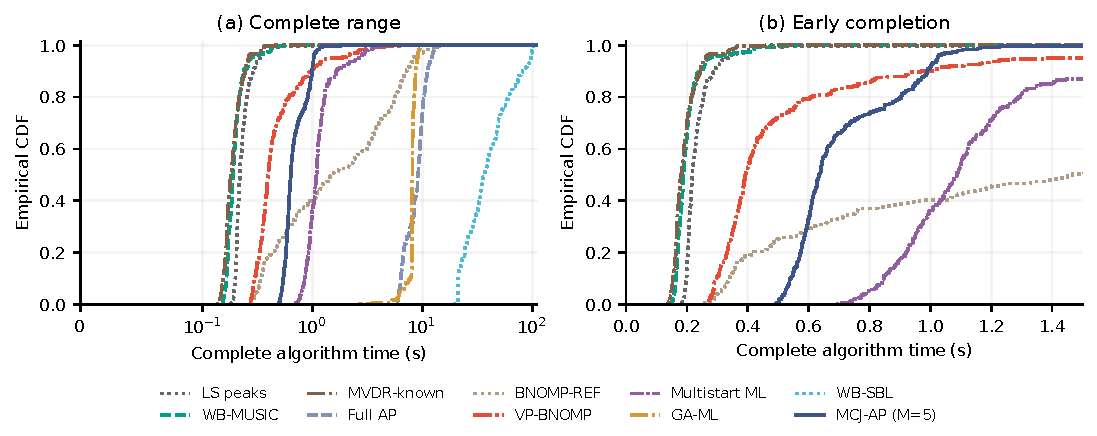
\includegraphics[width=\linewidth]{figures/assignment_cost_20261019/common_time_cdf.pdf}
\caption{与表\ref{tab:formalcommon}同批的完整耗时CDF。左图覆盖全部耗时，横轴0.1\,s内线性、其外对数；右图以线性坐标放大早期完成区间。}\label{fig:commontimecdf}
\end{figure}
\FloatBarrier
图\ref{fig:commontimecdf}显示，谱方法计算较快，但应结合误差CDF判断其定位质量。MCJ-AP在保持高恢复率的同时，比充分AP和SBL更早完成；VP-BNOMP多数观测较快，少量长循环使其耗时尾部超过MCJ-AP。因此，中位耗时与P95分别补充了典型成本和慢样本成本，不能只看平均值。


\section{功率差的构型分组结果}
功率差既可能影响正确区域内的定位精度，也可能改变候选选择。图\ref{fig:formalcore}将本批诊断发现的布局4与其余19布局分开，分别观察这两种影响。两组均保留全部随机实现、功率条件和失败结果，总体成绩见表\ref{tab:formalcore}。
\begin{figure}[pos=htbp]\centering
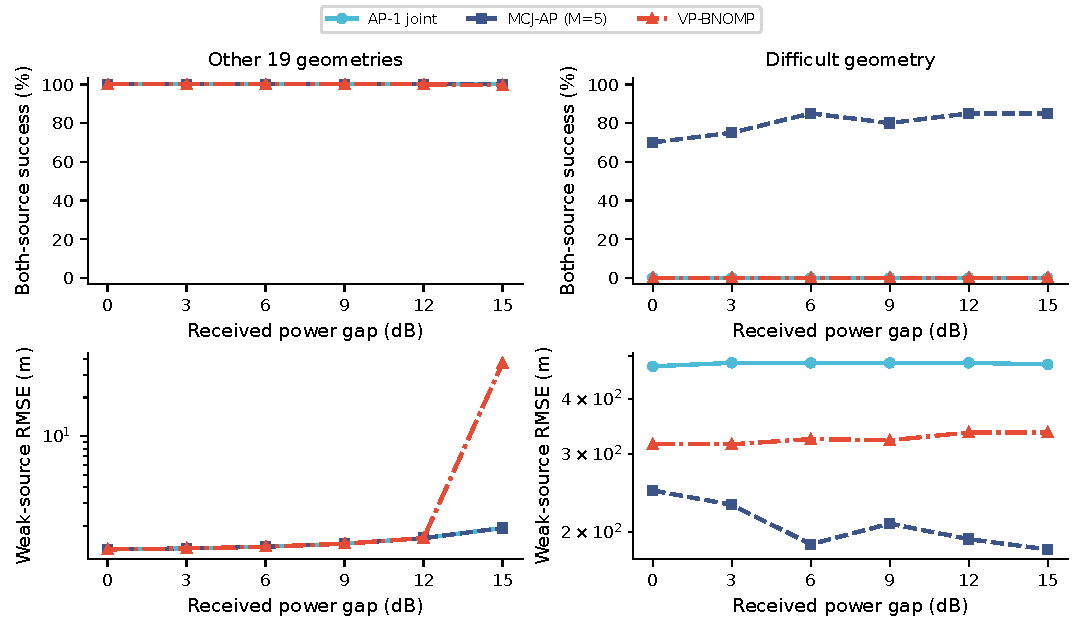
\includegraphics[width=.94\linewidth]{figures/formal_core.pdf}
\caption{扩展验证中功率差的分组结果。左列为其余19布局，共2280条、每档380条；右列为困难布局4，共120条、每档20条。上行为双源成功率，下行为弱源RMSE。分组依据本批构型诊断，全部2400条仍计入总体统计。}\label{fig:formalcore}
\end{figure}
\FloatBarrier
其余19布局中，两种AP均全部成功，MCJ-AP的弱源RMSE随功率差从1.31\,m增至1.93\,m，显示强源增强后弱源定位精度逐步下降。VP-BNOMP在这一组有两条15\,dB失败，因此该档RMSE仍受到长尾影响。右列单独呈现候选恢复困难，具体失败分布和候选机制在第\ref{sec:timecases}节集中分析。


\section{候选数量的耗时分布}
\begin{figure}[pos=htbp]\centering
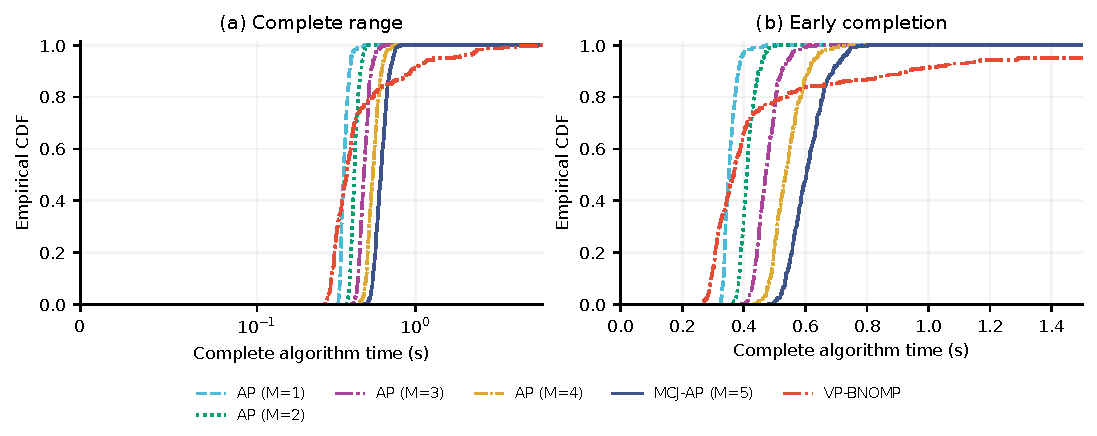
\includegraphics[width=\linewidth]{figures/assignment_cost_20261019/candidate_time_cdf.pdf}
\caption{同批240条观测的AP候选数与VP-BNOMP完整耗时CDF。每条曲线包含240条观测的完整求解耗时；左图0.1\,s内线性、其外对数，右图线性放大0--1.5\,s。}\label{fig:candidatetimecdf}
\end{figure}
\FloatBarrier
图\ref{fig:candidatetimecdf}中，增加AP候选数使耗时分布逐步右移。VP-BNOMP的中位耗时为0.3674\,s，接近单候选AP的0.3514\,s，但其耗时P95为1.3147\,s，高于五候选AP的0.7201\,s。两种流程的成本差别主要体现在分支数量和少量长循环，而不只是平均速度。


\section{局部更新的开发诊断}
为区分更新机制、停止尺度和数值保护的影响，采用四类开发构型、每类一个随机实现及0/15\,dB两档功率差，共8条观测作受控诊断。表\ref{tab:mechanism}中各变体只改变所列因素，候选发现和循环后共同LS保持一致。这组小规模对照用于解释机制，正式性能由后续共同240条及完整2400条结果评价。

\begin{table}[pos=H]\centering\small
\caption{局部更新的受控机制诊断。各版本使用相同8条开发观测；耗时包含必要预处理与求解，导数调用为每例均值。}\label{tab:mechanism}
\begin{tabular}{@{}lrrr@{}}\toprule
局部更新设置 & 双源成功 & 耗时/s & 导数调用\\\midrule
固定系数，能量容差$10^{-8}$ & 8/8 & 5.478 & 2679.5\\
仅放宽能量容差至$10^{-7}$ & 7/8 & 2.318 & 1133.9\\
仅放宽能量容差至$10^{-6}$ & 6/8 & 0.971 & 467.4\\
仅取消局部小步长退出 & 8/8 & 8.011 & 4758.4\\
局部波形消元，能量容差$10^{-8}$ & 8/8 & 0.436 & 70.4\\\bottomrule
\end{tabular}\end{table}

固定系数参照的21436次局部更新全部被接受，其中83.67\%的步长小于0.01\,m；Hessian正定修正、步长封顶、回溯缩步与边界裁剪均未触发。小步因此来自更新方向本身。放宽停止虽减少计算，却使部分弱源误差超过20\,m；取消小步长退出则增加了每轮内部计算。局部消元保留原能量容差，将平均导数调用由2679.5次降至70.4次。

相同位置与最小二乘系数下的曲率核对进一步解释了这一差别。在两个站外诊断位置，未施加数值保护的固定系数Newton试探步分别约0.0138\,m和0.0111\,m，消元试探步分别约11.25\,m和32.26\,m；这些试探方向用于比较曲率，实际接受步仍由回溯确定。四个保存位置的解析消元Hessian与自动微分结果的最大差约$1.4\times10^{-18}$。这与式\eqref{eq:schur}一致：允许波形随位置调整后，消元曲率去除了可由系数补偿的响应变化，减少了固定系数更新中的重复小步。


\section{时间轨迹与逐布局诊断}
\subsection{求解时间轨迹与困难构型的候选恢复}\label{sup:timecases}
图\ref{fig:formaltime}重放共同240条观测上已经保存的输出。尚无双源输出的观测按未成功计；RMSE仅在全部观测有输出后显示。
\begin{figure}[pos=htbp]\centering
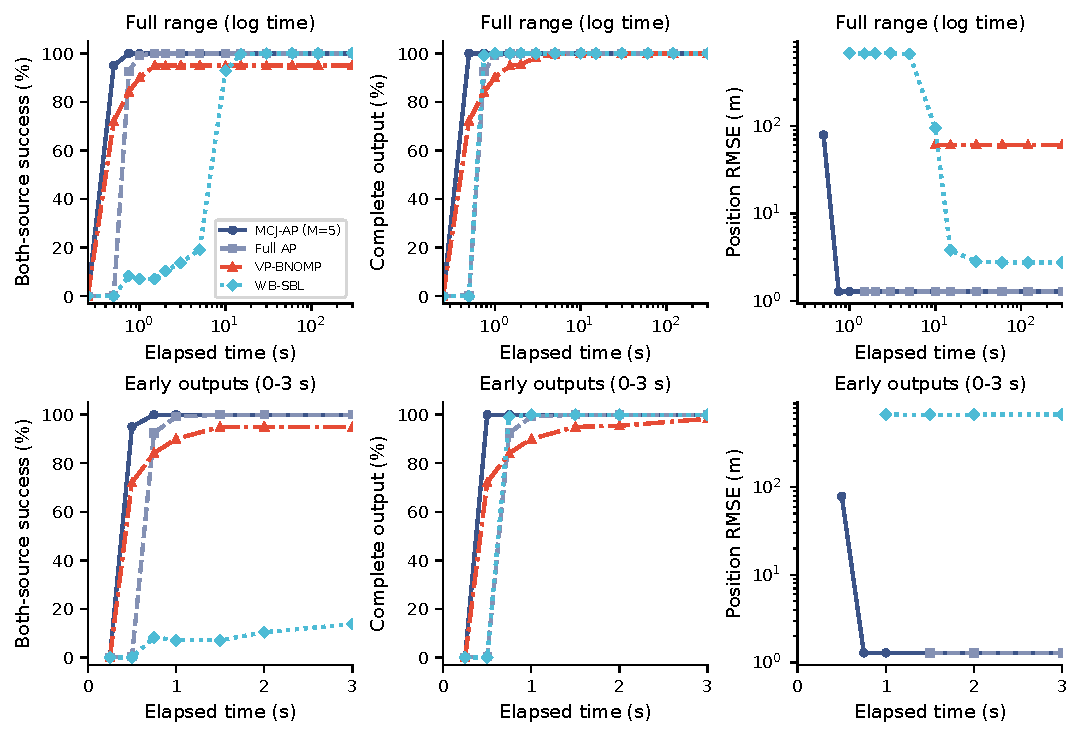
\includegraphics[width=\linewidth]{figures/formal_time.pdf}
\caption{共同240条观测的保存输出轨迹。上行使用0.25--300\,s对数时间轴，下行以线性时间轴放大0--3\,s；三列依次为双源成功率、完整输出比例和两源合并RMSE，后者为$\sqrt{(nK)^{-1}\sum_{i,k}e_{ik}^2}$。正常停止后保持最终值，RMSE纵轴仍用对数刻度。连接线表示保存点之间的变化，不额外规定算法停止时刻。}\label{fig:formaltime}
\end{figure}
\FloatBarrier

五候选联合AP、充分AP和SBL首次达到全部成功的保存点分别为0.75\,s、1.5\,s和30\,s。取得高质量结果的时间与完成全部计算的时间需要分别观察。上行对数轴便于比较亚秒至数百秒的差异，下行则分辨早期输出。VP-BNOMP在本次登记轨迹中只发布最终完整双源结果，其曲线不代表内部每次循环均已有对外输出。

\paragraph{困难构型下的候选覆盖}
图\ref{fig:formallayouts}给出全部20布局的失败分布，用于定位总体长尾的来源。
\begin{figure}[pos=htbp]\centering
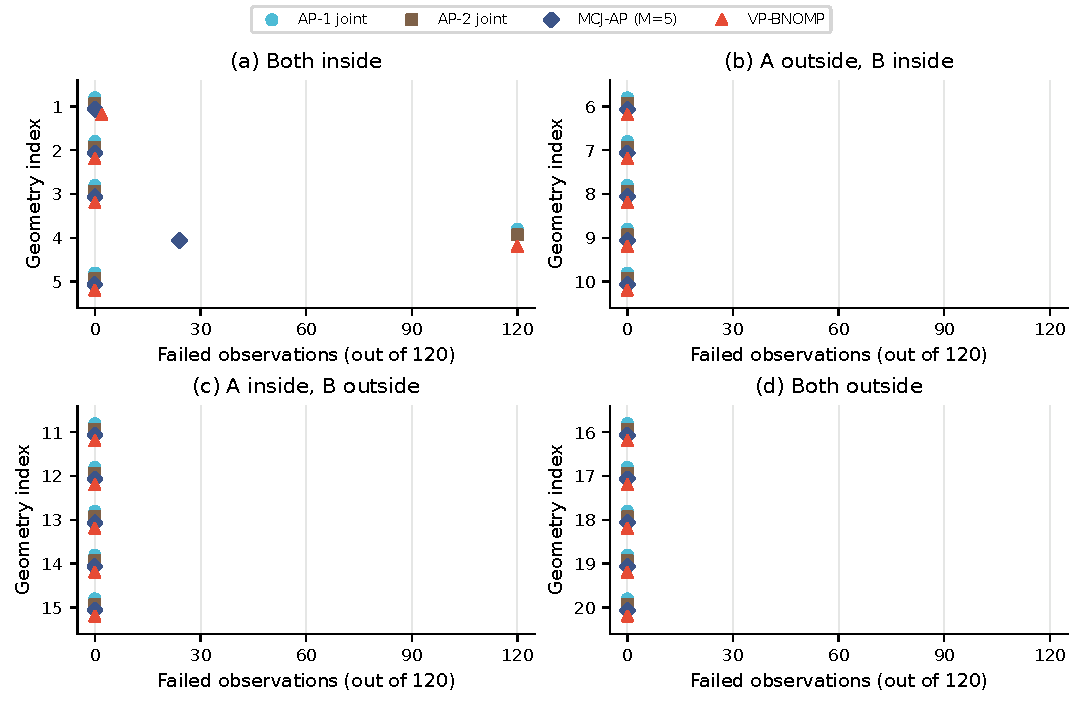
\includegraphics[width=\linewidth]{figures/formal_layouts.pdf}
\caption{各布局的双源失败数，每布局120条。四个面板对应四类构型，零表示该布局全部成功；不同标记在纵向稍作错开，便于辨认重合结果。}\label{fig:formallayouts}
\end{figure}
\FloatBarrier
单候选AP在布局4的120条观测上全部失败，五候选恢复其中96条；恢复涉及该布局20次随机实现中的18次，其余24条失败涉及6次实现，两组可包含同一实现的不同功率条件。其余19布局没有成功转失败。多候选的可靠性收益集中在这一源站构型，并在多次波形与噪声实现中重复出现；其恢复过程可由候选位置及精修后的目标变化解释。

逐一回读2400条观测的五个精修分支，2376条至少存在一个双源误差均不超过20\,m的分支，最终残差择优也恰好选中这2376条的成功分支。本批没有出现成功分支被最终排序排除的情况。其余24条的五个精修结果均未达标，说明剩余损失发生在获得成功分支之前；仅凭最终分支结果，尚不能进一步区分初始区域遗漏与局部优化未恢复。这里的分支成功标签仅用于离线诊断，不参与算法择优。

VP-BNOMP在布局4同样未达到20\,m门槛，但将该布局的弱源RMSE从单候选AP的479.66\,m降至325.07\,m，说明它减少了部分错误解的偏差。其余19布局中，AP的弱源RMSE约1.52\,m，VP-BNOMP因布局1的两次不同随机实现在15\,dB下失败，RMSE为15.25\,m。因此，VP相对单候选AP的总体RMSE收益主要来自布局4的严重错误减轻；五候选AP则进一步将其中96条恢复到20\,m内。总体误差、达标率与CDF分别刻画了这些不同的变化。

MCJ-AP每档400条观测中有3--6条失败，均来自布局4，并贡献各档超过99.7\%的弱源平方误差。该布局内候选选择的变化主导了总体RMSE折线的非单调起伏；其余19布局的曲线则更清楚地显示功率差对定位精度的影响。同一组布局在六档功率差中保持不变，这种起伏并非各档采用了不同构型。


\bibliographystyle{\PaperRoot template/cas-model2-names}
\bibliography{\PaperRoot references/references}
\end{document}
